\section{Dependency Definitions}
Before we discuss the design details of \texttt{BeeFlow}, we first formally define two types of dependency that are supported in \texttt{BeeFlow}. Although the offline dependency has been extensively studied and supported in previous works \cite{liu2015survey, altintas2004kepler, deelman2005pegasus, ogasawara2013chiron, zhao2007swift}, we include a formal definition here for clarification and comparison with in situ dependency. 

\subsection{Offline dependency}
When we have two tasks $A$ and $B$ with $B$ (offline) depending on $A$, then $B$ can only be launched after $A$ has finished all its work. As shown in \textbf{Fig. \ref{offline}}, logically a synchronization point must to be placed between the finishing point of task $A$ and the starting point of task $B$ to enforce this dependency.
\begin{figure}[h]
    \centering
    
    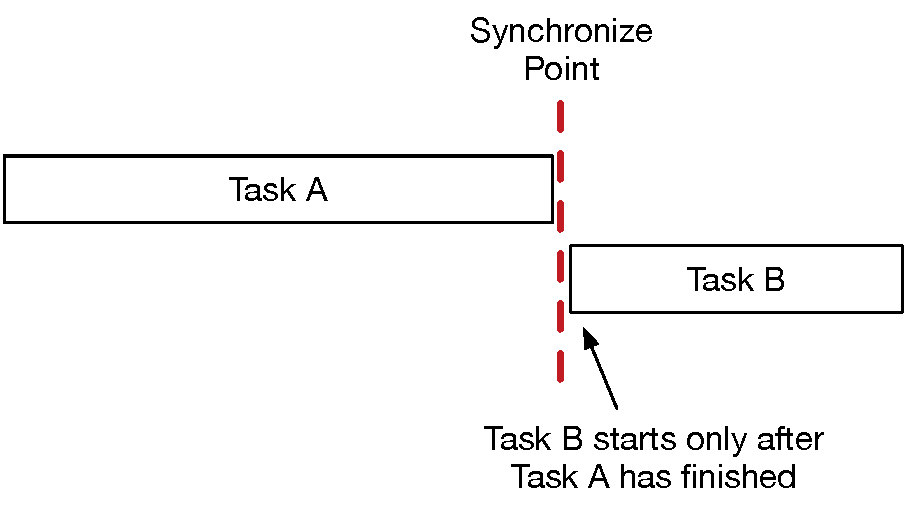
\includegraphics[width=0.45\textwidth]{figures/off-line.pdf}
    \caption{Example of offline dependency}
    \label{offline}
    
\end{figure}

\subsection{In situ dependency}
When we have two tasks $A$ and $B$ with $B$ (in situ) depending on $A$, then $B$ can be launched only after $A$ has started. As shown in \textbf{Fig. \ref{in situ}}, logically a synchronization point need to be placed in the beginning of task $A$ to enforce this dependency. The amount of time that task $B$ needs to wait after task $A$ starts can be defined according to application requirements.
\begin{figure}[h]
    \centering
   
    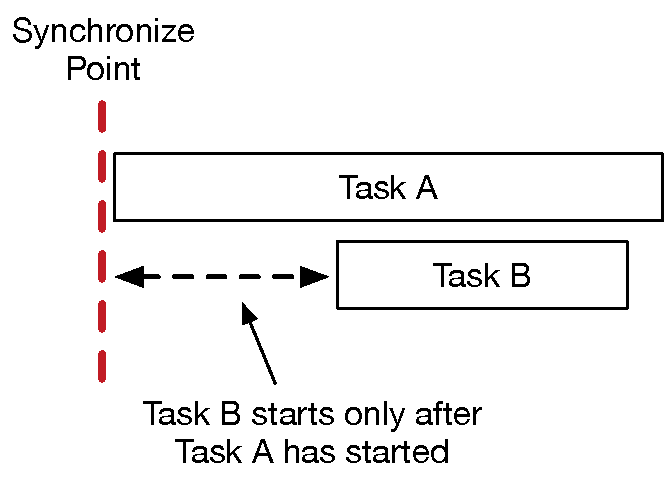
\includegraphics[width=0.35\textwidth]{figures/in-situ.pdf}
    \caption{Example of in situ dependency}
    \label{in situ}
    
\end{figure}

\section{Design}
Design of a scientific workflow management system usually follows the five-layer functional architecture model \cite{liu2015survey, altintas2004kepler, deelman2005pegasus, ogasawara2013chiron, zhao2007swift}. The five layers are:

\begin{itemize}
\item \textbf{Presentation Layer}:  This layer is responsible for gathering workflow information from the user and providing configuration capabilities.
\item \textbf{User Services Layer}: This layer is responsible for providing functionality (i.e., monitoring workflow status, etc.) to users.
\item \textbf{WEP Generation Layer}: This layer is responsible for generating the Workflow Execution Plan (WEP) based on the workflow design provided by the user in the presentation layer.
\item \textbf{WEP Execution Layer}: This layer is responsible for scheduling workflow tasks within the WEP.
\item \textbf{Infrastructure Layer}: This layer is responsible for managing underlaying infrastructures and executing workflow tasks on them.
\end{itemize}
\begin{figure}[h]
    \centering
    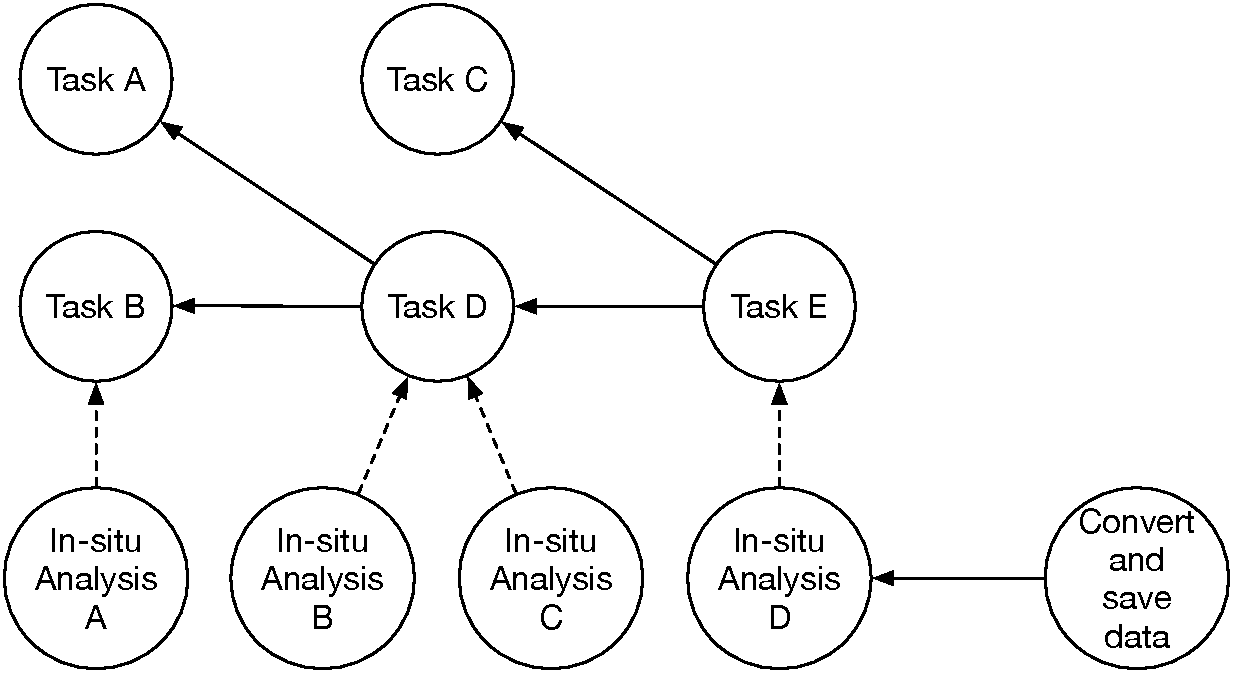
\includegraphics[width=0.45\textwidth]{figures/dag.pdf}
    \caption{Example of DAG with both offline and in situ dependency}
    \label{dag}
    
\end{figure}

\subsection{Presentation Layer}
Traditional offline-based dependency relations are usually represented using Directed Acyclic Graphs (DAGs). Tasks are represented as vertices and dependencies between them are represented as directed edges. We also choose DAG for dependency representation in \texttt{BeeFlow}. To incorporate in situ dependency into a DAG-based dependency representation, we extend DAG to use two types of directed edges to represent two types of dependencies: one for offline dependency (solid edges) and another for in situ dependency (dashed edges). We use a simplified example to show how the extended DAG represents workflow with both kinds of dependencies. In our example workflow, we have three different simulation tasks: \texttt{Task B}, \texttt{Task D}, and \texttt{Task E}. One simulation's input depends on another, so they have to be executed in order (i.e., offline dependency). Also, \texttt{Task D} and \texttt{Task E} need additional input, which need to be per-processed by \texttt{Task A} and \texttt{Task C} first (i.e., offline dependency).  Meanwhile, we also want to monitor the progress of each simulation with in situ analysis tools. \texttt{Task D} also has two separate in situ analysis tasks monitoring two different parts of the output of \texttt{Task D}. Finally, we want to convert and save the in situ analysis data for \texttt{Task E} after its in situ analysis task (\texttt{In-situ Analysis D}) has finished. This workflow mixes both traditional offline dependencies and in situ dependencies. We can represent its dependencies using our extended DAG as in \textbf{Fig. \ref{dag}}. Solid edges represent offline dependency and dashed edges represent in situ dependency.

DAGs are usually represented as a series of dependencies in workflow configuration files, the input files of workflow management tools. To represent both offline and in situ dependencies, we add an additional flag to indicate which mode is used. In our \texttt{Beeflow} management system, the description file is defined using JSON format. For example, the DAG of our example workflow is represented as follows:


\begin{lstlisting}[language=json,firstnumber=1,basicstyle=\small]
{
  "Task A": { 
    "dependency_list":[]
  },
  "Task B": { 
    "dependency_list": []
  },
  "Task C":{  
    "dependency_list": []
  },
  "Task D":{  
    "dependency_list": ["Task A", "Task B"],
    "dependency_mode": "Offline"
  },
  "Task E":{  
    "dependency_list": ["Task C", "Task D"],
    "dependency_mode": "Offline"
  },
  "In-situ Analysis A":{ 
    "dependency_list": ["Task B"],
    "dependency_mode": "In-situ" 
  },
  "In-situ Analysis B":{ 
    "dependency_list": ["Task D"],
    "dependency_mode": "In-situ"
  },
  "In-situ Analysis C":{ 
    "dependency_list": ["Task D"],
    "dependency_mode": "In-situ"
  },
  "In-situ Analysis D":{ 
    "dependency_list": ["Task E"],
    "dependency_mode": "In-situ"
  },
  "Convert and save data":{ 
    "dependency_list": ["In-situ Analysis E"],
    "dependency_mode": "Offline"
  }  
}
\end{lstlisting}


\subsection{User Services Layer}
In this section, we discuss the design details of how we build \texttt{BeeFlow} on top of \texttt{BEE} to provide workflow launching and monitoring features for users. 

When using the original \texttt{BEE} execution framework, users first need to start the \texttt{BEE Orchestration Controller} in the background. The orchestration controller is responsible for handling task launching requests. To launch tasks, users need to use the \texttt{BEE launcher} to send task launching requests to the \texttt{BEE Orchestration Controller}. However, the original design only allows one task to be launched at a time. To launch a multi-task workflow, users need to manually launch each task and carefully handle complicated dependencies between them. 

To enable workflow launching features, we need to extend \texttt{BEE} to launch multiple tasks. The simplest and most straightforward design is to modify the \texttt{BEE launcher}, allowing it to group multiple task launching requests into one. Since the \texttt{BEE Orchestration Controller} was originally designed to handle one task at a time, tasks in a multiple task launching request will still be handled one by one, sequentially. So, it would significantly degrade launching efficiency, especially for tasks that will pull large Docker images. On the other hand, a more efficient way to enable multiple task support is to handle multiple task launching requests simultaneously, so they will not interfere or block each other. Inspired by the commonly used web server design, in which each client's request is handled by an individual thread, we modify \texttt{BEE Orchestration Controller} to handle multiple task launching requests following similar design principles. 


The launching workflow of our extended \texttt{BEE Orchestration Controller} is as follows: First, when the \texttt{BEE Orchestration Controller} receives task launching requests and related task information, instead of starting the launching process immediately on the main thread, the \texttt{BEE Orchestration Controller} now creates several new \texttt{BEE} task threads and stores all related task information to the thread object including status indicator variables for querying their launching and execution progress later. Then, BEE task threads are launched. The \texttt{BEE Orchestration Controller} uses a hash table to store all task threads with the task name as the key for locating tasks quickly. At anytime, users can launch a separate monitoring tool to keep track of the status of all the tasks they are running. In addition, as we will discuss in later sections, we install event-based listeners to each \texttt{BEE} task thread to enforce task dependencies during task launching. The overall framework of our extended BEE Orchestration Controller is shown in \textbf{Fig. \ref{orc}}. We create a special launcher, \texttt{BeeFlow Composer}, dedicated for launching workflows with multiple tasks. 

\begin{figure}[h]
    \centering
    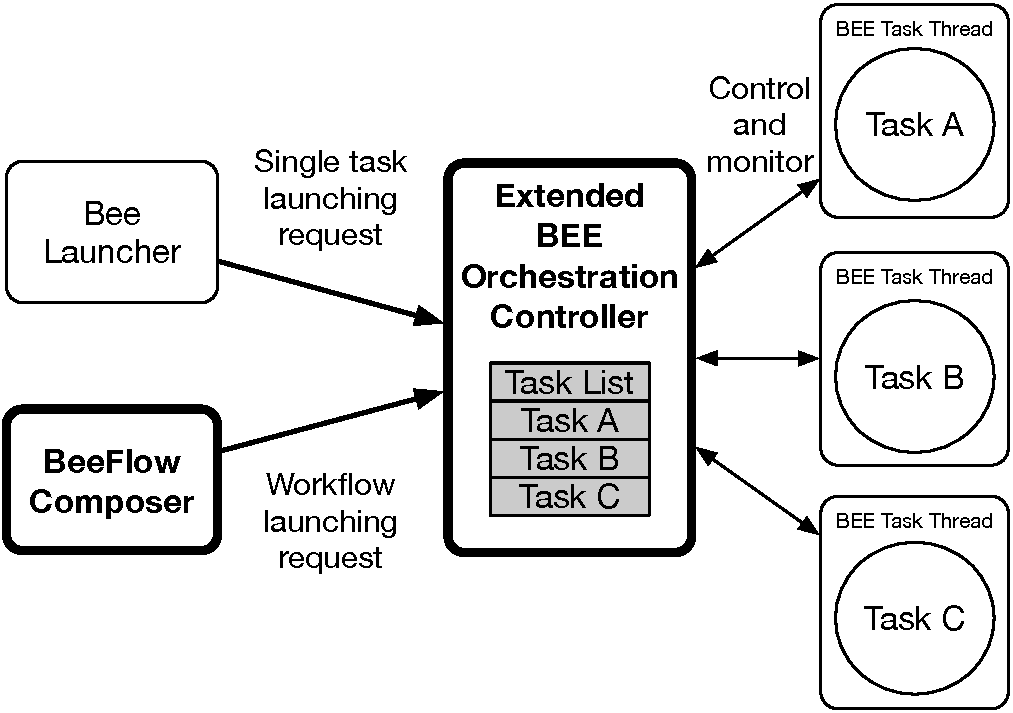
\includegraphics[width=0.4\textwidth]{figures/orc_ctl.pdf}
    \caption{Extended BEE Orchestration Controller with multiple task handling capabilities}
    \label{orc}
    
\end{figure}

\subsection{WEP Generation Layer}
The next step is to generate WEPs, which include all task-related preparation before actual execution. Specifically, besides creating \texttt{BEE} task threads as mentioned in the previous section, we also need to provision each \texttt{BEE} task thread to enforce the workflow logic specified by users while launching tasks. 

First, we need to get the task launching order from our previously defined JSON formatted workflow dependency description file. For traditional pure offline dependency mode, we can get the task launching order using Topology Sort from a series of dependencies. To incorporate both offline and in situ dependency mode, we find that it is hard to use Topology Sort, since in situ dependency mode allows both tasks to be started at the same time and cannot be described as a series of launching orders. Instead we propose to use primitive synchronization elements in Python to enforce this kind of mixed launching order. During the creation of each \texttt{BEE} task thread, we create two Python event objects: one for sending out signals when the task starts and another for sending out signals when the task finishes. Other tasks can listen for these signals to enforce dependencies. 

\textbf{Algorithm \ref{top}} shows the algorithm used to add Python event objects for enforcing workflow logic. For each task in the \texttt{Beeflow} workflow description file, we check if it is in some other tasks' dependency list. If so, the dependent task is set to wait for the event signals from those tasks according to the dependency type.

\begin{algorithm}
\caption{\texttt{Beeflow} launching logic}
\label{top}
\begin{algorithmic}[1]
\REQUIRE{Task List (TL)}
\FOR{task in TL}
	\STATE create two events: start\_event, end\_event;
	\FOR{task2 in TL}
		\IF{task in task2.dependency\_list}
			\IF{task2.dependency\_mode == "in situ"}
				\STATE task2.add\_wait\_for (start\_event);
			\ENDIF
			\IF{task2.dependency\_mode == "offline"}
				\STATE task2.add\_wait\_for (end\_event);
			\ENDIF
    	\ENDIF
      \ENDFOR 
\ENDFOR
\end{algorithmic}
\end{algorithm}

\textbf{Fig. \ref{exp}} shows how Python event objects are added to our previous workflow example to enforce launching orders. Each rectangle represents a simplified launching source code of each task. $S*$ and $E*$ represent event objects for starting and ending the current task. The \texttt{wait for} function will block the current task's launching process until all of the events it is waiting for have received signals. Notice \texttt{Task A} to \texttt{Task E} are on the offline workflow, so each one of them needs to wait for the end signal sent from certain tasks. The four in situ analysis processes are in in situ dependency mode, so they wait for the start signals of corresponding simulation tasks. Finally, \texttt{Convert and save data} in the end must wait for the completion of \texttt{In-situ Analysis D}; so, it waits for its end signal.
\begin{figure}[h]
    \centering
    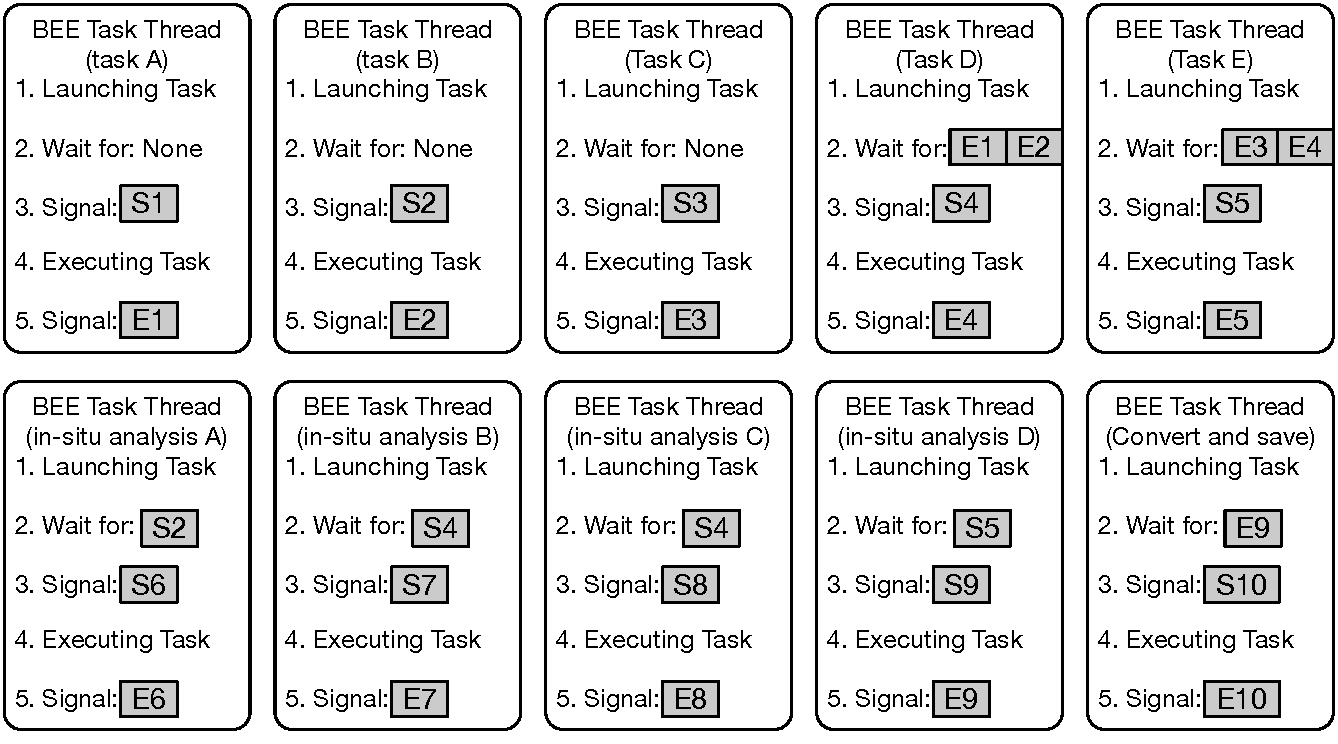
\includegraphics[width=0.45\textwidth]{figures/exp.pdf}
    \caption{Example of applying events synchronization primitive to enforce workflow logics}
    \label{exp}
    
\end{figure}


\subsection{WEP Execution Layer}
Once task threads are constructed and configured with dependency enforcement event objects, they are ready for launching. The launching is handled by \texttt{BEE}. Depending on users' configuration, workflow tasks can run on HPC systems or AWS platforms. Since events objects are integrated into each task, no modification is necessary to \texttt{BEE} to run workflow-related tasks, and \texttt{BEE} is not aware of the dependencies between tasks. So, \texttt{BEE} schedules \texttt{BeeFlow} tasks the same as regular tasks (i.e., as if no dependencies exist) and workflow dependencies can be enforced by each task. This design simplifies the launching process and eliminates overhead brings by task progress monitoring for dependencies enforcement purposes as in other workflow tools. 

\subsection{Infrastructure Layer}
\subsubsection{Execution}
Basically, each task is executed by \texttt{BEE} on different platforms specified by users. To provide a unified environment across platforms, \texttt{BEE} uses a Docker container as it's execution environment. On HPC platforms, \texttt{BEE} uses its universal back-end \texttt{BEE-VM} to run Docker. On AWS, \texttt{BEE} can directly use BOTO API to launch pre-built Docker-enabled instances then run the user applications within the Docker container. 

\subsubsection{DataFlow Design}

\begin{comment}
\begin{figure*}[h]
    \centering
    \caption{Example of using SSH tunnel for in situ analysis workflow}
    \label{tunnel}
    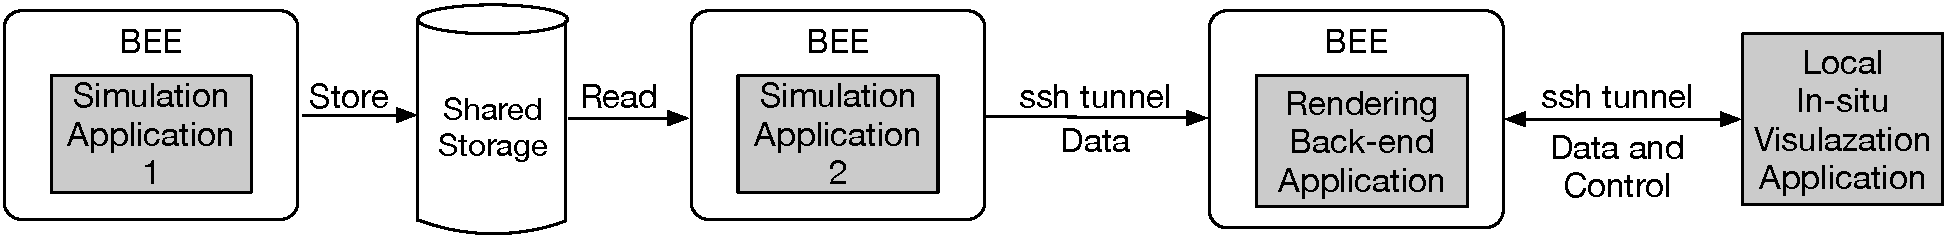
\includegraphics[width=0.8\textwidth]{figures/tunnel.pdf}
\end{figure*}
\end{comment}
In workflow, data are usually produced by some tasks and then consumed by other tasks. This is the reason dependencies exist. For in situ analysis, the analysis tools sometimes control the simulation processes. In this section, we discuss the dataflow design in \texttt{BeeFlow} to support these functionalities.

First, we design the traditional disk-based dataflow between tasks in \texttt{BeeFlow} where one task writes output to files on disk and another reads the files as input data. We assume file names are predefined in both tasks in order to allow data sharing between tasks, we need to make sure both tasks can access the same working directory or a synchronized directory. In \texttt{BEE}, the task applications run in Docker containers, and data is mounted with two steps: (1) a shared local directory (on HPC systems) or shared EFS (on AWS) is mounted to a pre-configured directory in BEE-VM or BEE-AWS. (2) the pre-configured directory is mounted into the working directory in the Docker container. In order to share the same working directory between two dependent tasks, we only need to ensure that they are mounting the same local directory or EFS, which can be configured before launch in \texttt{BEE}. 

The second kind of dataflow is socket-based dataflow, in which data is transfered between tasks using TCP/UDP sockets. As a simulation task progresses, it sends out data to in situ analysis tools for processing. Later, as shown in the Flecsale workflow of our case study, as the simulation makes progress and sends out data, users can employ local ParaView clients to visualize simulation progression. Socket connections can be easily established when user tasks are running on bare metal systems. However, when using \texttt{BEE}, the execution environment is isolated between tasks. Modification to the network configuration of the two-layer virtulization is difficult. So instead we propose to use the existing SSH connections to establish tunnel connections between tasks, since it requires minimum modification to \texttt{BEE} and avoids all complicated configurations by users. Moreover, the tunnel connection not only allows data transfer from simulation application to in situ analysis tools, it also allows backward simulation control from the in situ analysis tool (e.g., ParaView Catalyst \cite{ahrens2005paraview, ayachit2015paraview}).

